
\chapter{CLMR}\label{sec:method}
\begin{quote}
    In this chapter, the core components of the CLMR framework are detailed. The data augmentation pipeline is outlined, as well as the evaluation procedure of the representations learned by CLMR. Concluding, the transfer learning experiments are explained.
\end{quote}

The following core components of the framework are outlined in the following sections:
\begin{itemize}
    \item A stochastic composition of data augmentations that produces two correlated, augmented examples of the same audio segment, the `positive pair', denoted as $x_i$ and $x_j$.
    This is done for all segments in the mini-batch, resulting in $2N$ augmented examples per mini-batch.
    \item An encoder neural network $g_{\mathrm{enc}}(\cdot)$ that encodes the augmented examples to their latent representations.
    \item A projector neural network $g_{\mathrm{proj}}(\cdot)$ that maps the encoded representations to the latent space where the contrastive loss is formulated.
    \item A contrastive loss function, which aims to identify $x_j$ from the negative examples in the mini-batch $\{x_{k\neq i}\}$ for a given $x_i$.
\end{itemize}

The complete framework is visualised in Figure \ref{fig:clmr_model}.

\begin{figure*}[h]
    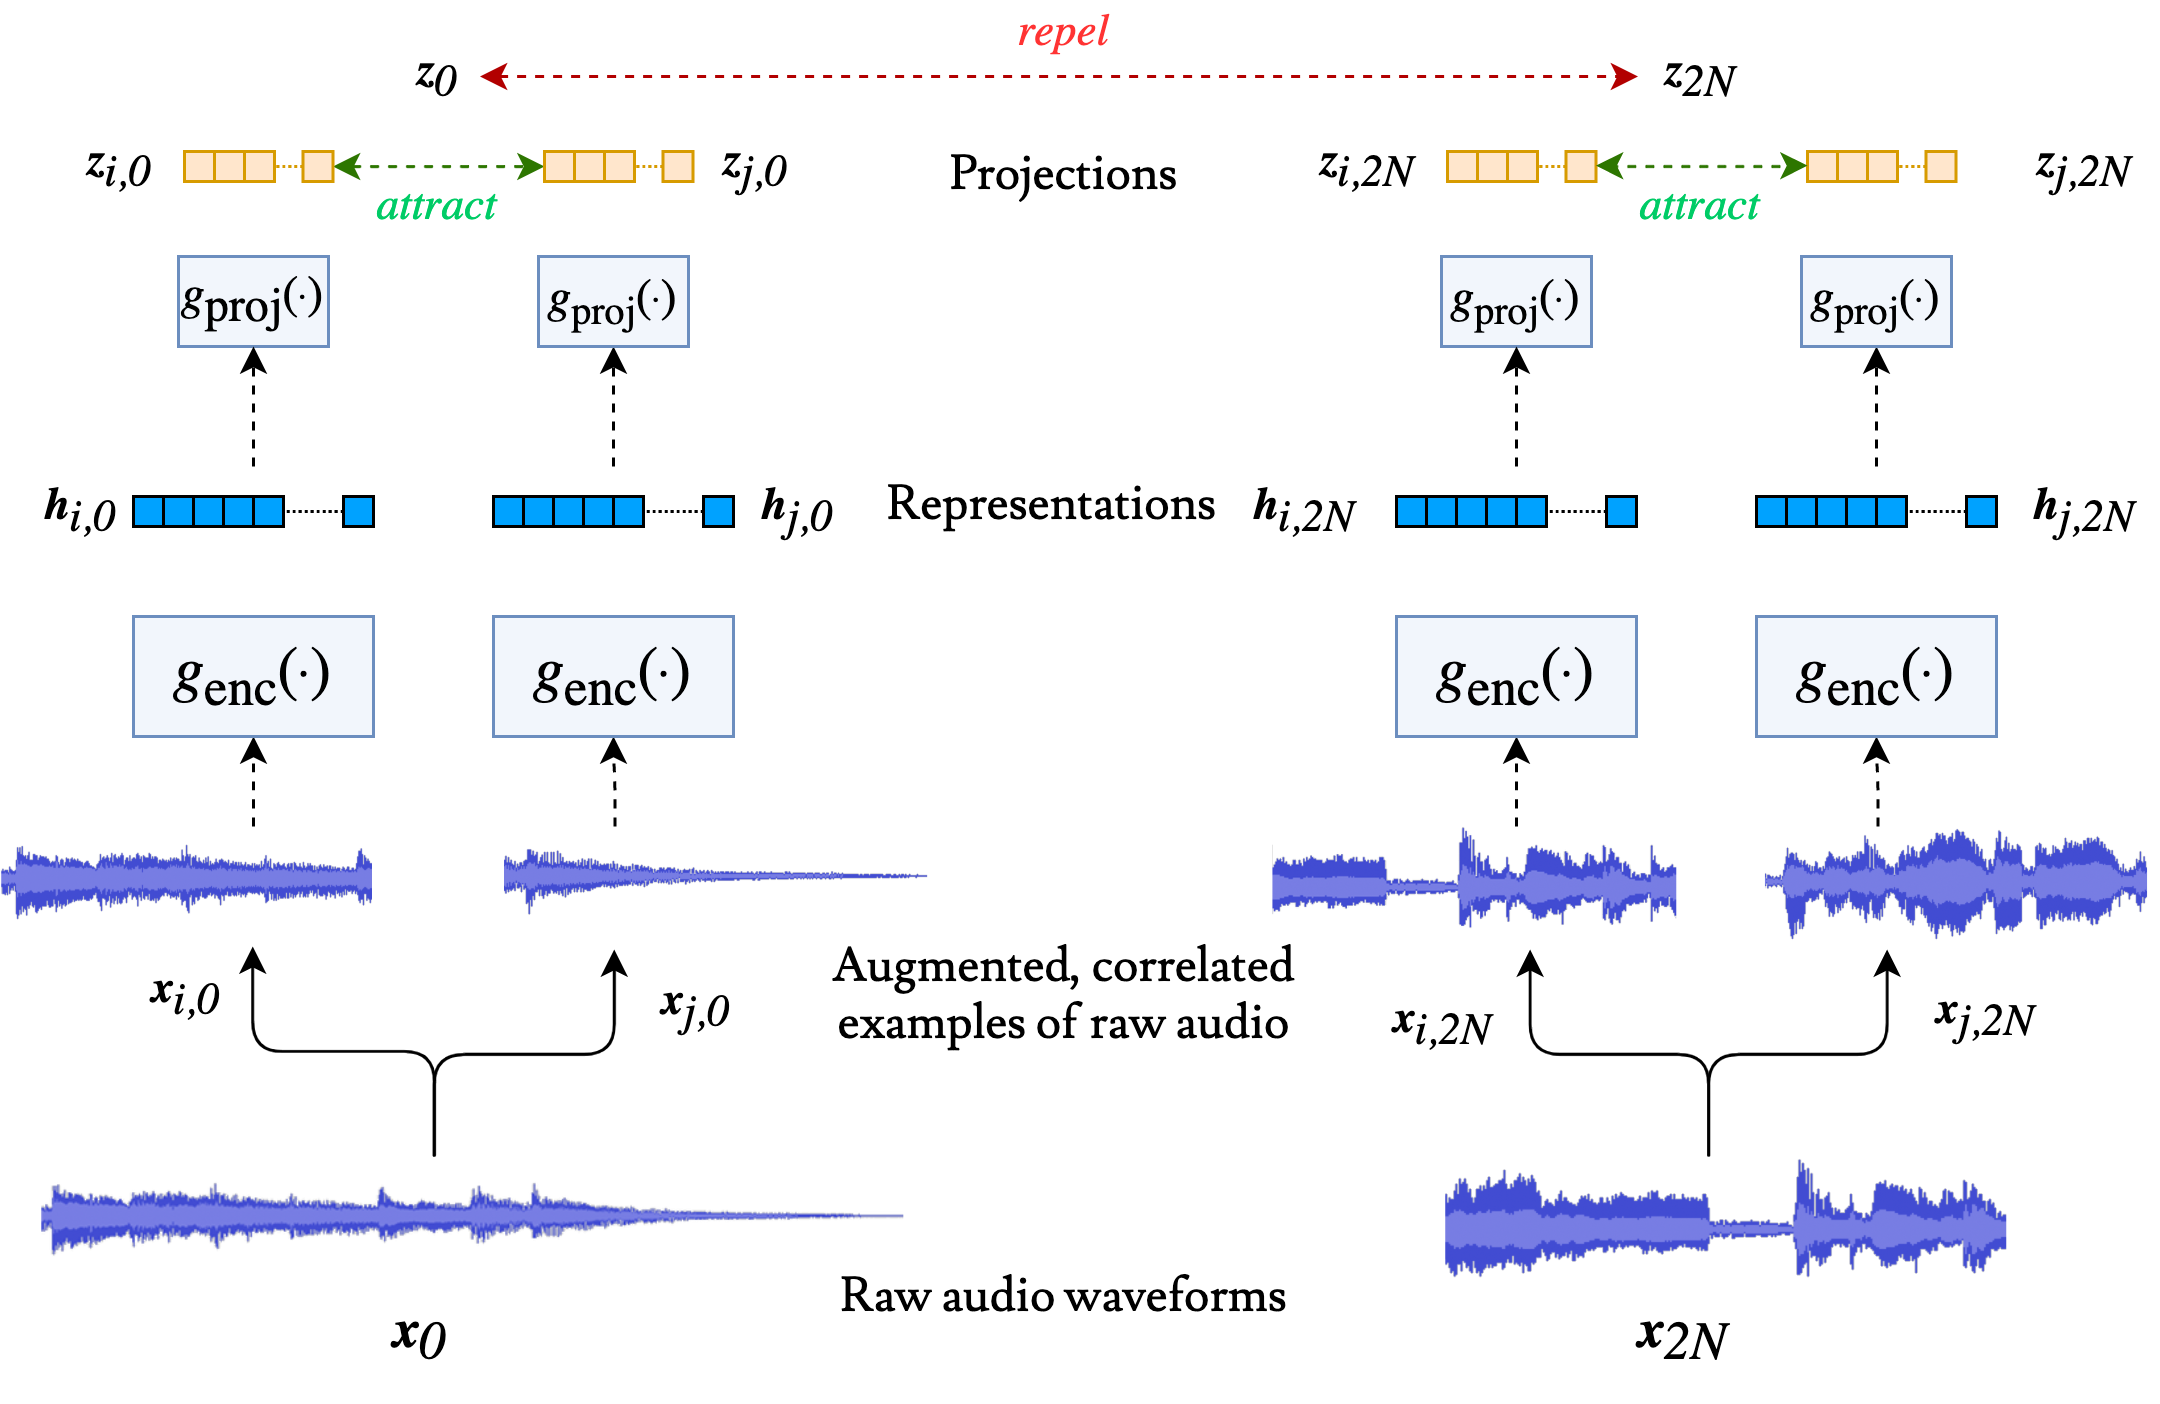
\includegraphics[width=\columnwidth]{figs/clmr_model.png}
    \caption{The CLMR framework operating on raw audio, in which the contrastive learning objective is directly formulated in the latent space of correlated, augmented examples of pairs of raw audio waveforms.}
    \label{fig:clmr_model}
\end{figure*}

\section{Data Augmentations}
We designed a chain of augmentations for raw audio waveforms to make it harder for the model to identify the correct pair of examples.
The following augmentations were applied on ${x_i}$ and ${x_j}$ independently:
\begin{enumerate}
    \item A random segment of size $N$ is selected from a full piece of audio, without trimming silence (e.g., the intro or outro of a song).
    The independently chosen segments for $x_i$ and $x_j$ could overlap or be very disjoint, allowing the model to infer both local and global structures. This intuition is visualised in Figure \ref{fig:global_local}.
    \item The polarity of the audio signal is inverted, i.e., the amplitude is multiplied by $-1$, with probability $p_{\mathrm{invert}}$.
    \item Additive White Gaussian Noise is added with a high signal-to-noise ratio to the original signal with probability $p_{\mathrm{noise}}$.
    \item The gain is reduced between $[-6, 0]$ decibels with probability $p_{\mathrm{gain}}$.
    \item A filter is applied with probability $p_{\mathrm{filter}}$.
    A coin flip determines whether it is a low-pass or a high-pass filter. The cut-off frequencies are randomly drawn from the uniform distribution $[2200, 4000]$ or $[200,1200]$ respectively.
    \item The signal is delayed with probability $p_{\mathrm{delay}}$.
The delay time is randomly chosen from values between 200-500ms, with 50ms increments.
The volume factor of the delayed signal that is added to the original signal is 0.5.
    \item The signal is pitch shifted with probability $p_{\mathrm{pitch}}$.
The pitch transposition interval is drawn from a uniform distribution consisting of intervals ranging from a fifth below to a fifth above the original signal's scale.
    \item Reverb is added to the signal with probability $p_{\mathrm{reverb}}$.
The impulse response's room size, reverbation and damping factor is randomly chosen from a uniform distribution of values between $[0-100]$.
\end{enumerate}
The space of augmentations is not limited to these operations and could easily be extended to, e.g., randomly applying chorus, distortion and other modulations, as outlined in Section \ref{sec:audio_transformations}.



\begin{marginfigure}
    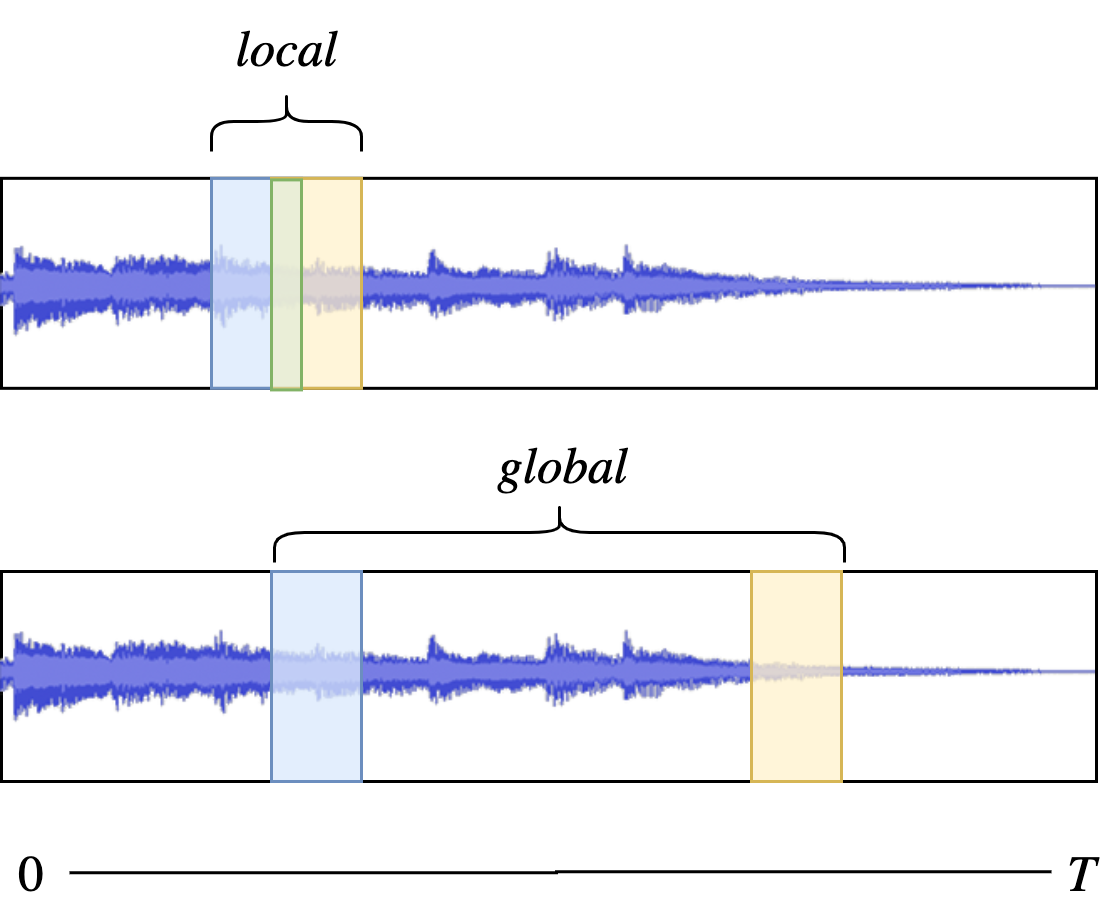
\includegraphics[width=\textwidth]{figs/clmr_local_global.png}
    \caption{...}
    \label{fig:global_local}
\end{marginfigure}



\section{Mini-Batch Composition} % Negative examples
We sample one song from the mini-batch, augment it into two examples, and treat them as the positive pair.
We treated the remaining $2(N-1)$ examples in the mini-batch as negative examples, and did not sample the negative examples explicitly.
A larger batch size makes the model's objective harder -- there are simply more negative samples the anchor sample needs to identify the positve samle from -- but it can substantially improve model performance \cite{chen_simple_2020}.
This introduces a practical problem for raw audio when training on a GPU, as the input dimensionality of a raw waveform is higher for high sample rates.
The batch size can be increased more easily when audio is re-sampled at lower sampling rates: the number of examples the model is exposed to at once can be higher when the number of audio samples is lower.

Alternatively, multiple GPU's can be used for training, but this introduces another practical problem: batch normalisation \cite{batch_normalisation} is used in the encoder to stabilise training.
When training in a distributed, parallel manner, the batch normalisation statistics (mean/variance) are usually aggregated locally per device.
Positive examples are sampled on the same device, leading to potential leakage of batch statistics which improves training loss, but counteracts learning of useful representations.
We used global batch normalisation, which aggregates the batch statistics over all devices during parallel training, to alleviate this issue. We leave the effect of different stabilisation strategies, e.g., layer normalisation \cite{henaff2019data}, for future work.


\section{Encoder}
To directly compare a state-of-the-art end-to-end supervised model against a self-supervised model operating on raw waveforms, we use the SampleCNN model as our encoder \cite{lee2018samplecnn}.
Similar to the supervised approaches, we use an audio input of 59\,049 samples for audio with a sample rate of 22\,050~Hz.
In this configuration, the SampleCNN encoder $g_{\mathrm{enc}}$ consists of 11 blocks, each with a convolutional layer with a filter size of 3, batch normalisation, ReLU activation and max pooling with pool size 3.
The fully connected and dropout layers are removed, yielding a 512-dimensional feature vector for every sample of audio.
This feature vector is subsequently mapped to a different latent space by the projector network $g_{\mathrm{proj}}$ where the contrastive loss function is defined.
We adjust the audio input length and the encoder's blocks according to the configurations proposed in \cite{lee2018samplecnn} when training on audio sampled at different sampling rates (16\,000, 12\,000 and 8\,000~Hz).

% There is a trade-off between the number of contrastive examples the model is exposed to at once, and model complexity: increasing both quickly results in hardware constraints for training (GPU memory).
We found working with a batch size of 48, i.e., 96 samples per batch since we use $2N$ samples for our negative sampling strategy, and the $3^9$-SampleCNN encoder configuration to work well and easier to compare with against related work using supervised methods \cite{lee2018samplecnn, dieleman2014end,pons_end--end_2017}.
We leave model scaling for future work.


\section{Projector}
The feature vectors from the encoder can be directly used in the learning objective, but SimCLR shows that formulating the objective on encodings mapped to a different latent space by a parameterised function helps the effectiveness of the representations \cite{chen_simple_2020}.
We evaluate the performance improvement when using a linear layer $z_i = Wh_i$, non-linear layer $z_i = W^{(2)}\operatorname{ReLU}(W^{(1)}h_i)$ and an identity function $z_i = h_i$ as the projector.
% \diffword{Layer2 is data augment in \ref{clmr}}.


\section{Contrastive Loss Function}
In keeping with recent findings on several objective functions in contrastive learning \cite{chen_simple_2020}, the contrastive loss function used in this model is normalised temperature-scaled cross-entropy loss, commonly denoted as \emph{NT-Xent loss}:
\begin{equation}
    \label{ntxent_loss}
    \ell_{i, j}=-\log \frac{\exp \left(\operatorname{sim}\left(z_{i}, z_{j}\right) / \tau\right)}{\sum_{k=1}^{2 N} \mathbbm{1}_{[k \neq i]} \exp \left(\operatorname{sim}\left(z_{i}, z_{k}\right) / \tau\right)}
\end{equation}
%, demonstrated for a single pair in equation \ref{ntxent_loss}.

Instead of using a scoring function that preserves the mutual information between vectors, the pairwise similarity is measured using cosine similarity ($\operatorname{sim}$).
% : $f(\cdot) = \operatorname{sim}(\boldsymbol{u}, \boldsymbol{v})=\boldsymbol{u}^{\top} \boldsymbol{v} /\|\boldsymbol{u}\|\|\boldsymbol{v}\|$.
It introduces a new temperature parameter $\tau$ to help the model learn from hard negatives.
The indicator function $\mathbbm{1}_{[k \neq i]}$ evaluates to $1$ iff $k\neq i$.
% ref to figure
This loss is computed for all pairs, both $(z_i, z_j)$ and $(z_j, z_i)$, resulting in the following total loss function:
% shown in equation \ref{total_xent_loss}.

\begin{equation}
    \label{total_xent_loss}
    \mathcal{L} = \frac{1}{2N}\sum_{i=1}^{N}\sum_{j=1}^{N} \mathbbm{1}_{[i\neq j]}\ell_{i, j}
\end{equation}

We used the Adam optimizer \cite{adam_optimizer} with a learning rate of $3\times10^{-4}$ and train until convergence.


\section{Evaluation}
\label{evaluation}
The evaluation of representations learned by self-supervised models is commonly done with linear evaluation \cite{oord_representation_2019,hjelm_learning_2019,chen_simple_2020}, which measures how linearly separable the relevant classes are under the learned representations.
We obtain representations $h_t$ for all data points $X$ from a frozen CLMR network after pre-training has converged, and train a linear classifier using these self-supervised representations on the downstream task of music classification.
For CPC, the representations are extracted from the autoregressor, yielding context vector $c$ of $256$ dimensions, which is global-average pooled to obtain a single vector of $512$ dimensions.
For CLMR, the representations $h$ from the encoder are used instead of the representations $z$ from the projector.


\section{Transfer Learning}
To test the generalisability of the learned representations, we also pre-trained CLMR on different datasets than those we use for fine-tuning.
We pre-train CLMR on the Million Song Dataset, freeze the weights of the network, and subsequently process all datapoints $X$ from the smaller MagnaTagATune dataset to obtain representations $h$, on which we perform the same linear evaluation procedure outlined in the previous paragraph.
